\documentclass[border=3pt,tikz]{standalone}
\usepackage{amsmath}
\usetikzlibrary{arrows}
\usetikzlibrary{positioning}
\usetikzlibrary{calc}
\usetikzlibrary{arrows}
\usetikzlibrary{decorations.pathreplacing}
\begin{document}
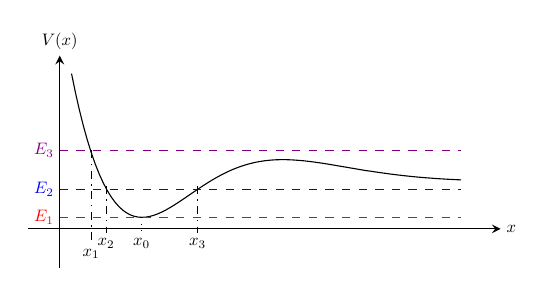
\begin{tikzpicture}[domain=1.05:6, samples = 100, scale=1]

    \draw[-{stealth}] (0.5, 0) -- (6.5,0) node[right, scale=0.6] {$x$};
    \draw[-{stealth}] (0.9,-0.5) -- (0.9,2.2) node[above, scale=0.6] {$V(x)$};
    
    \draw[color=black]   plot[id=veff] (\x, {2* ( (\x * \x) - (4 * \x) +  3 + (1 * (\x^-1)))  * exp(-0.2* (\x^2)) + 0.6 } ) ;
    \draw[dashed, red] (0.9, 0.15) node[left, scale=0.6] {$E_1$}-- (6.0, 0.15) ;
    \draw[dashed, blue] (0.9, 0.5) node[left, scale=0.6] {$E_2$}-- (6.0, 0.5) ;
    \draw[dashed, violet] (0.9, 1.0) node[left, scale=0.6] {$E_3$}-- (6.0, 1.0) ;
    \draw[dashdotted] (1.3, 1.0) node[above, scale=0.6] {$$} -- (1.3, -0.18) node[below, scale=0.6] {$x_1$};
    \draw[dashdotted] (1.49, 0.55) -- (1.49, -0.05) node [below, scale=0.6] {$x_2$};
    \draw[dashdotted] (2.65, 0.55) -- (2.65, -0.05) node [below, scale=0.6] {$x_3$};
    
    \draw[dotted] (1.94, 0.15) -- (1.94, -0.05) node [below, scale=0.6] {$x_0$};
    
    \end{tikzpicture}
\end{document}